\chapter{Measurements}
\section{Narrow Band Transmission}
\label{sec:res_450}

First a relatively narrow signal transmitting at only a quarter
of the maximal symbol rate was build and analyzed to show some basic
properties of the system and to show what the best achievable
\gls{EVM} values are. \\

As receiver architecture, the Quadrature Intermediate Frequency Sub-Nyquist
Sampling Receiver as described in \secref{sec:rx_2} is used with the difference
that the signal bandwith is only $B = 450 MHz$. All the other properties are listed
in \tblref{tab:res_450}. \\

\begin{table}[h]
  \centering
  \begin{tabular}{|l|r@{}l@{~}l|}
    \hline
    $f_{\text{TX IF}}$ & 2&.9&GHz \\ \hline
    $f_{\text{TX LO}}$ & 57&.5&GHz \\ \hline
    $f_{\text{RX LO}}$ & 58&.2&GHz \\ \hline
    $f_{\text{RX IF}}$ & 2&.2&GHz \\ \hline
    $f_c$            & 60&.4&GHz \\ \hline
    Signal Bandwidth B & 0&.45&GHz \\ \hline
    Sample Rate $f_s$ & 1&.8&GHz \\ \hline
  \end{tabular}
  \caption{Properties of Narrow Band Transmission System}
  \label{tab:res_450}
\end{table}

\subsection{Measurement Setup and RF System Analysis}
A block diagram providing an overview of the test setup,
used for all following measurements, can be found in \figref{fig:res_450_bd}. \\

\begin{figure}[p]
  \centering
  %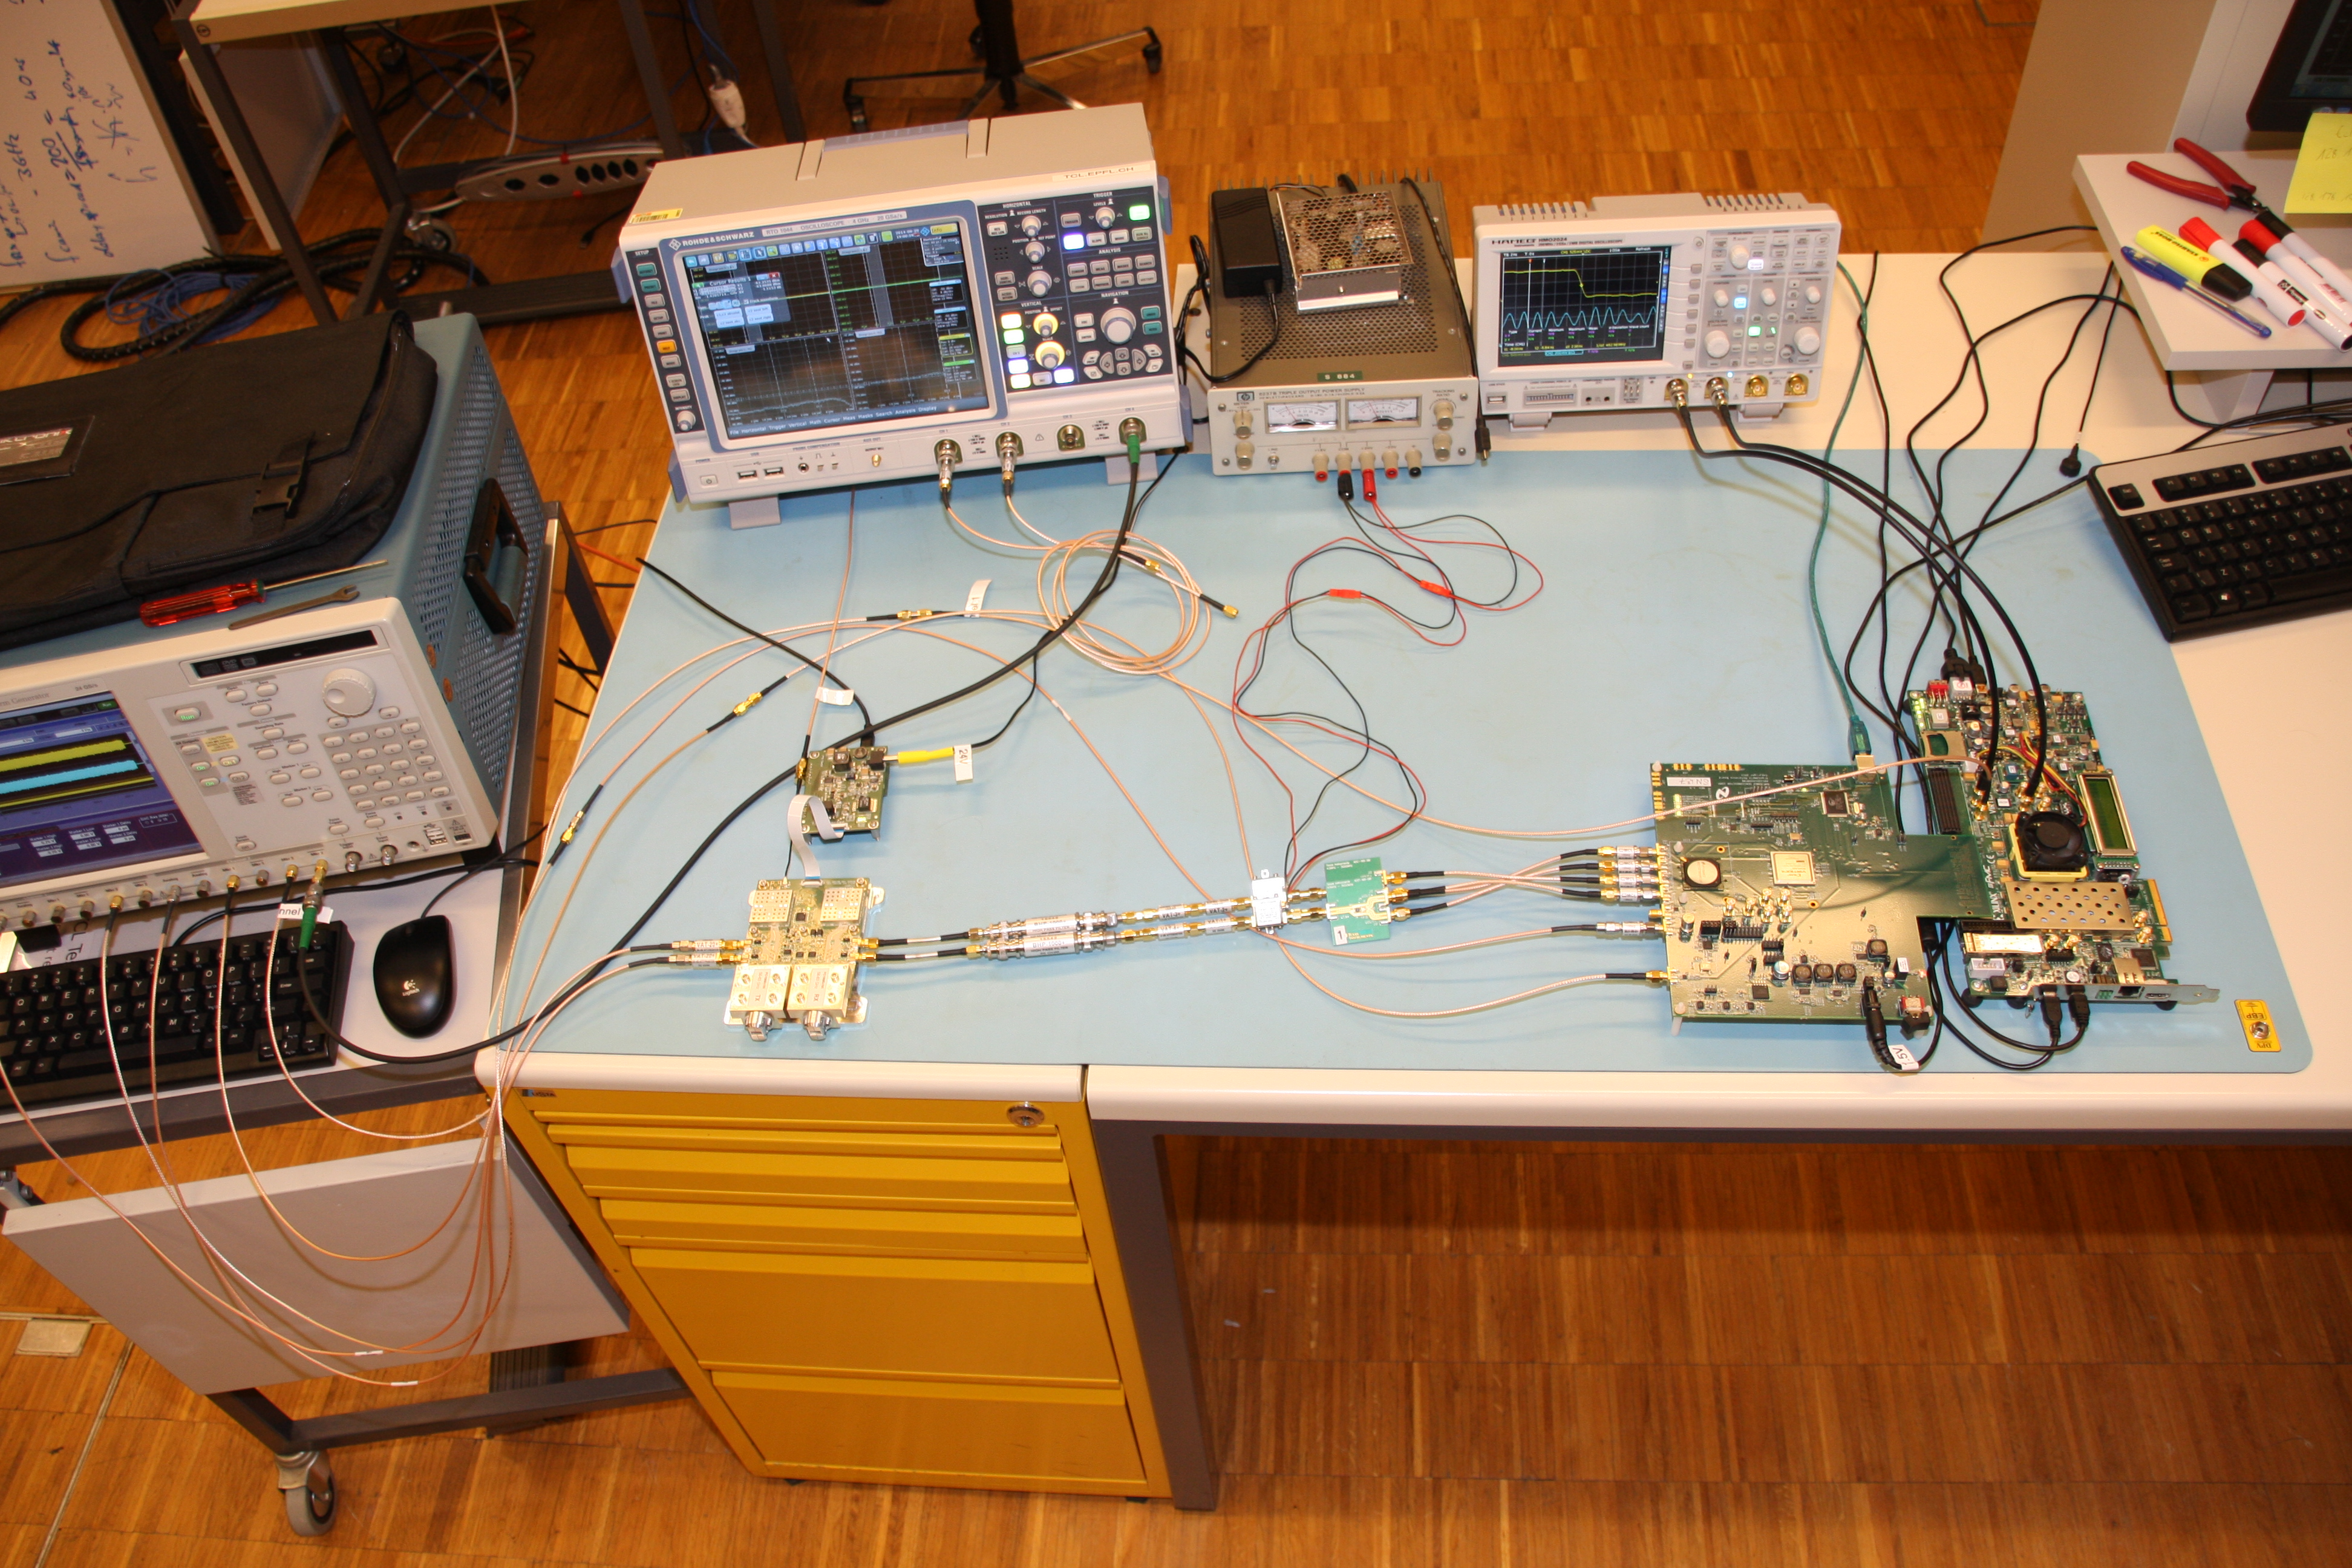
\includegraphics[width=\textwidth]{pictures/res_450_setup}
  \caption{Block Diagram of the Narrow Band Transmission Setup}
  \label{fig:res_450_bd}
\end{figure}
\todo{draw block diagram}

\begin{figure}[p]
  \centering
  %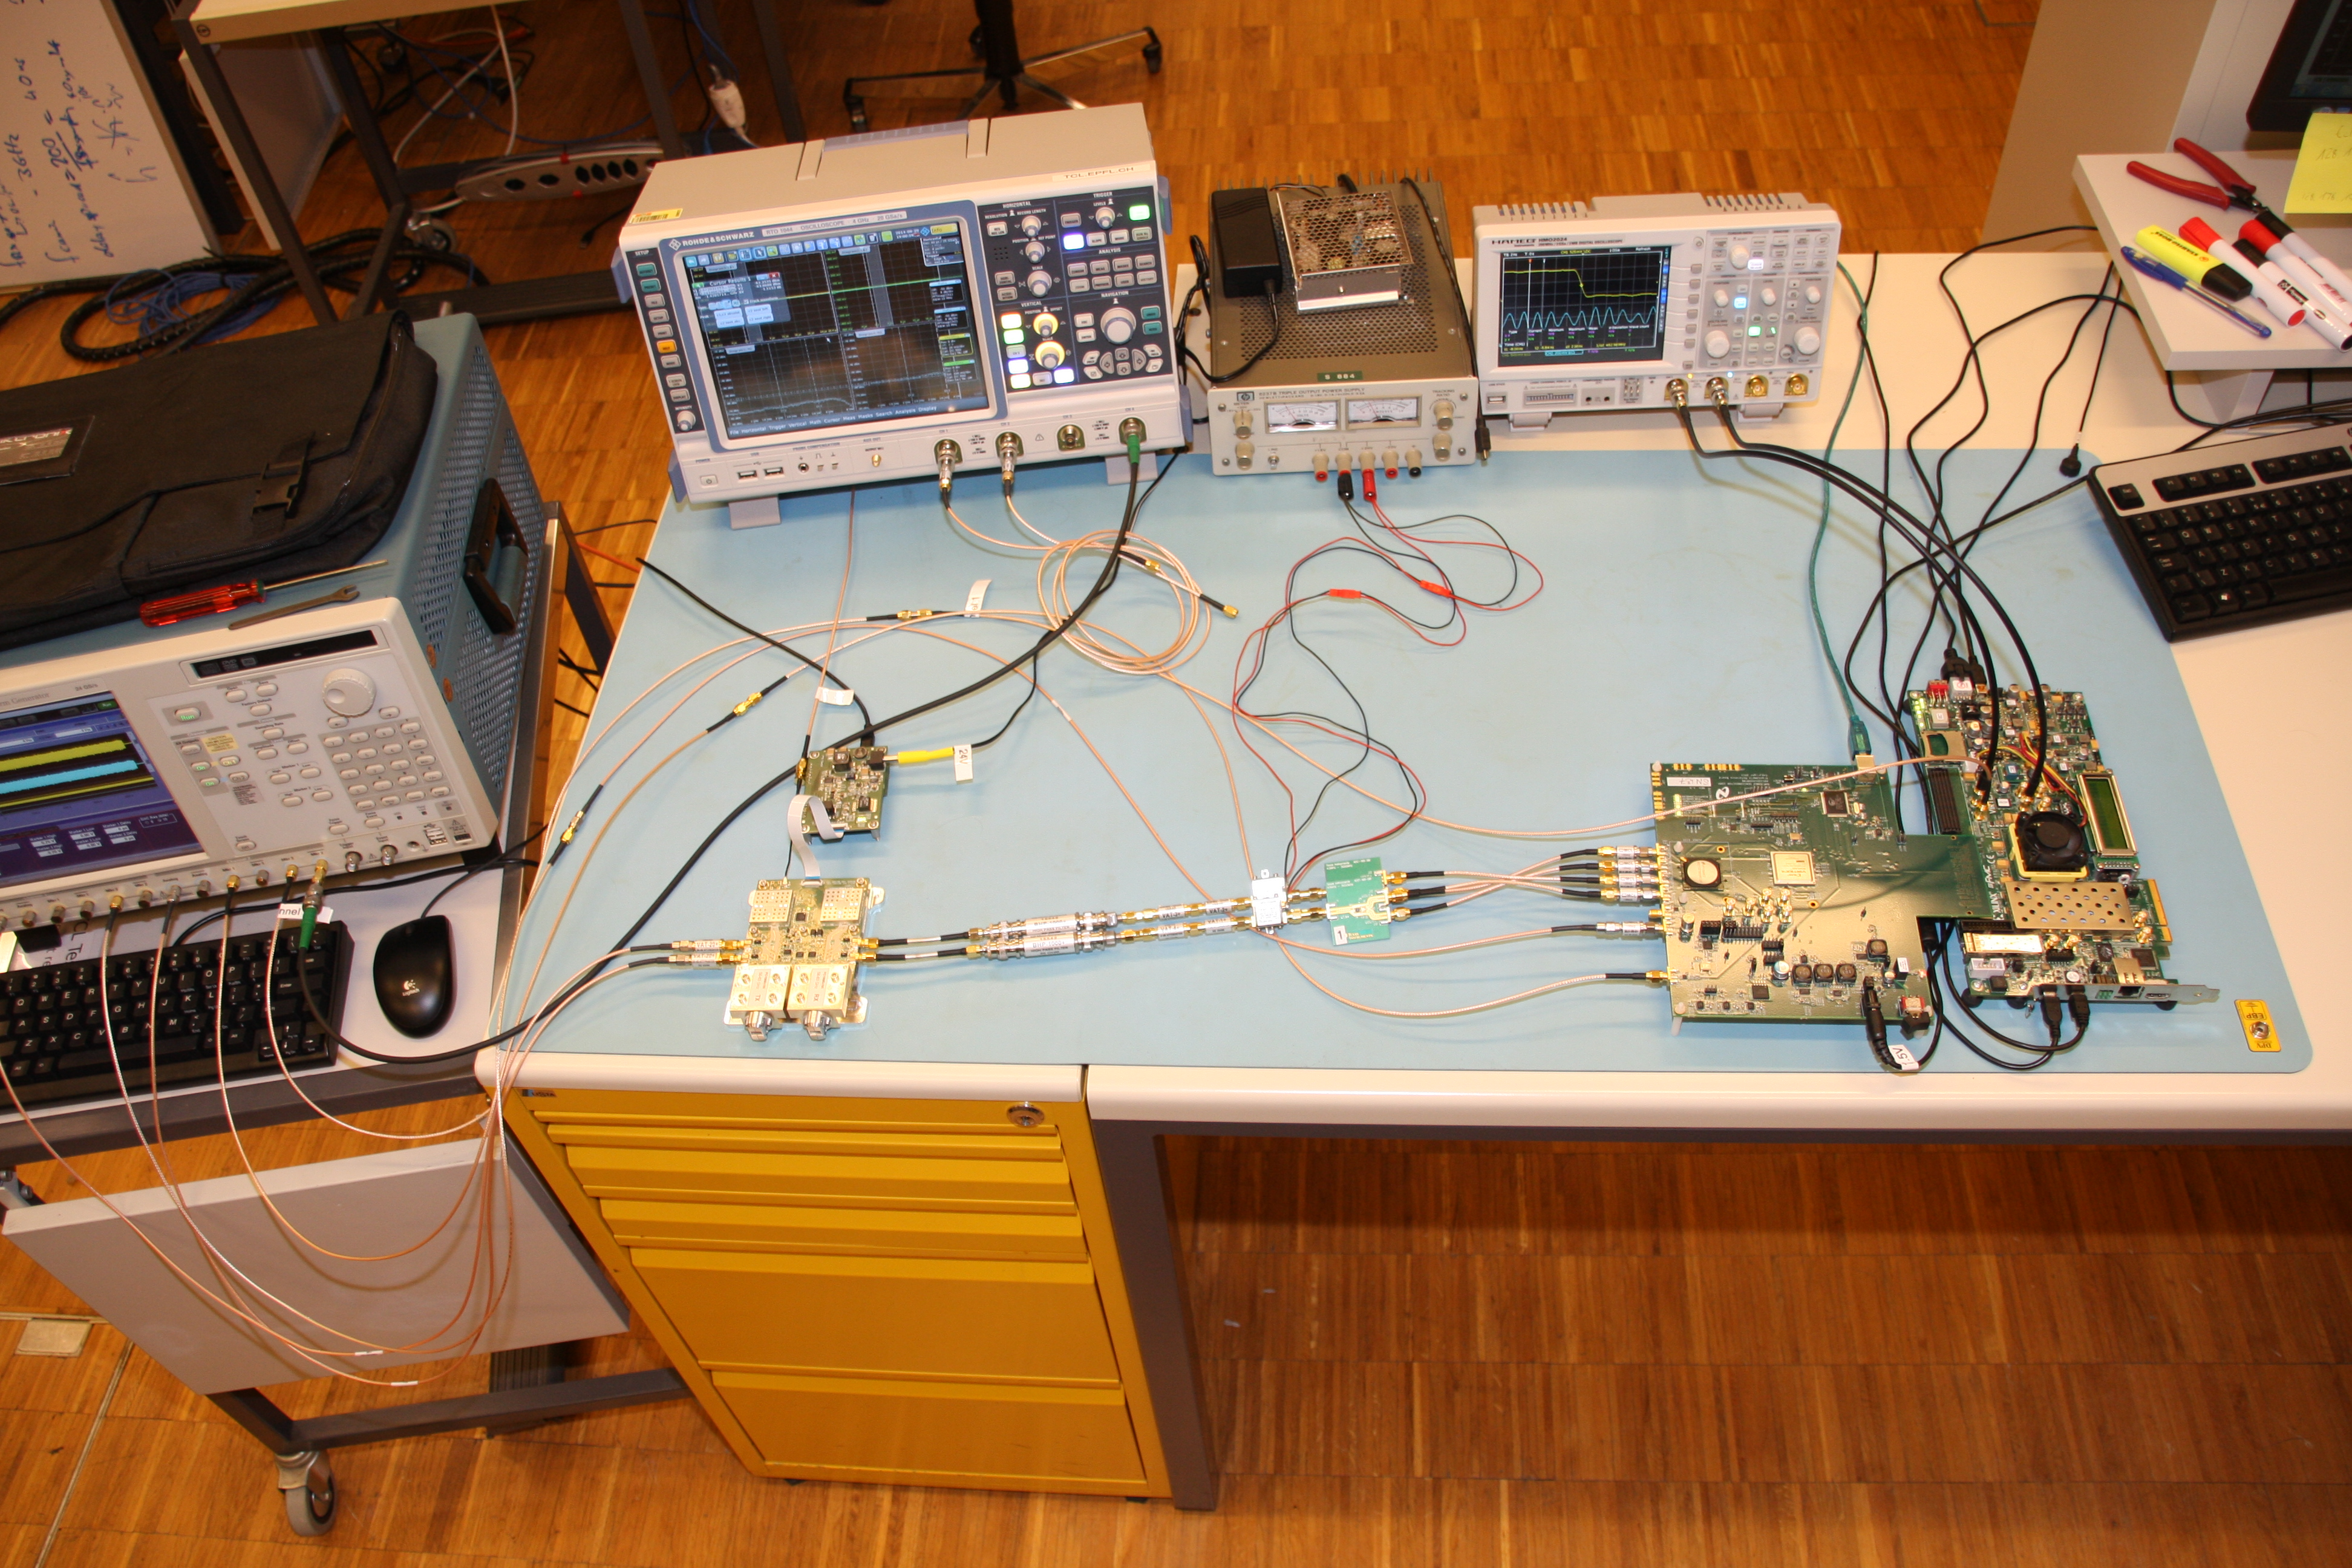
\includegraphics[width=\textwidth]{pictures/res_450_setup}
  \caption{Picture of the Narrow Band Transmission Setup}
  \label{fig:res_450_pic}
\end{figure}

\subsubsection{Matlab}
The Matlab script was configured such that it generates the transmitt signal,
programs the \gls{AWG}, reads the data acquired by the \gls{FPGA},
runs the receiver code and finally generets reports and figures. \\
The configuration file used for these tests can be found in
\appref{app:res_450_cnf}. \\

\subsubsection{\gls{AWG}}
The \gls{AWG} was configured to output the \gls{TX} \gls{IF} signal $i[k]$,
the sample clock for the \gls{ADC} as well as synchronization pulses to trigger
the \gls{FPGA} and oscillocope. It's configuration and port assignment
are shown in \tblref{tab:res_450_awg}.

It was noticed, that the used \gls{AWG} has some cross talk from
channel 1 marker 1 output to the channel 1 analog output. Therefor the
\gls{ADC} clock should always be output on marker 2 and not on marker 1.
For synchronization pulses, this is not an issue, since they are ware always
configured to give a 100 cycle wide positive pulse $> 100 \text{ns}$ before
the signal starts. \\

\begin{table}[h]
  \centering
  \begin{tabular}{|l|l|}
    \hline
    Sampling Rate & 10.8 GS/s \\ \hline
    Clock Source & Externals 10 MHz \\ \hline
    Analog Amplitude & 1 $\text{V}_{\text{pp}}$ \\ \hline
    Marker Amplitude CH1 Marker 1/2 & 0, 0.7 V \\ \hline
    Marker Amplitude CH2 Marker 1/2 & 0, 1.4 V \\ \hline
    \gls{DAC} resolution & 8 bit \\ \hline
    CH 1 & $i[k]$ \\ \hline
    CH 2 & $\mathcal{H}\{i[k]\}$ \\ \hline
    CH 1 Marker 1 & 0 \\ \hline
    CH 1 Marker 2 & 1.8 GHz \gls{ADC} sample clock \\ \hline
    CH 2 Marker 1 / 2 & Sync pulse before frame starts \\ \hline
  \end{tabular}
  \caption{Configuration and Port Assignment of \gls{AWG}}
  \label{tab:res_450}
\end{table}

An osilloscope plot (see \secref{sec:comp_osci}) of the generated
\gls{TX} \gls{IF} signal and it's \gls{FFT} can be found in
\figref{fig:res_450_awg_analog}.
The \gls{ADC} clock signal and the sync pulse are shown
in \figref{fig:res_450_awg_digital}. \\

\begin{figure}[p]
  \centering
  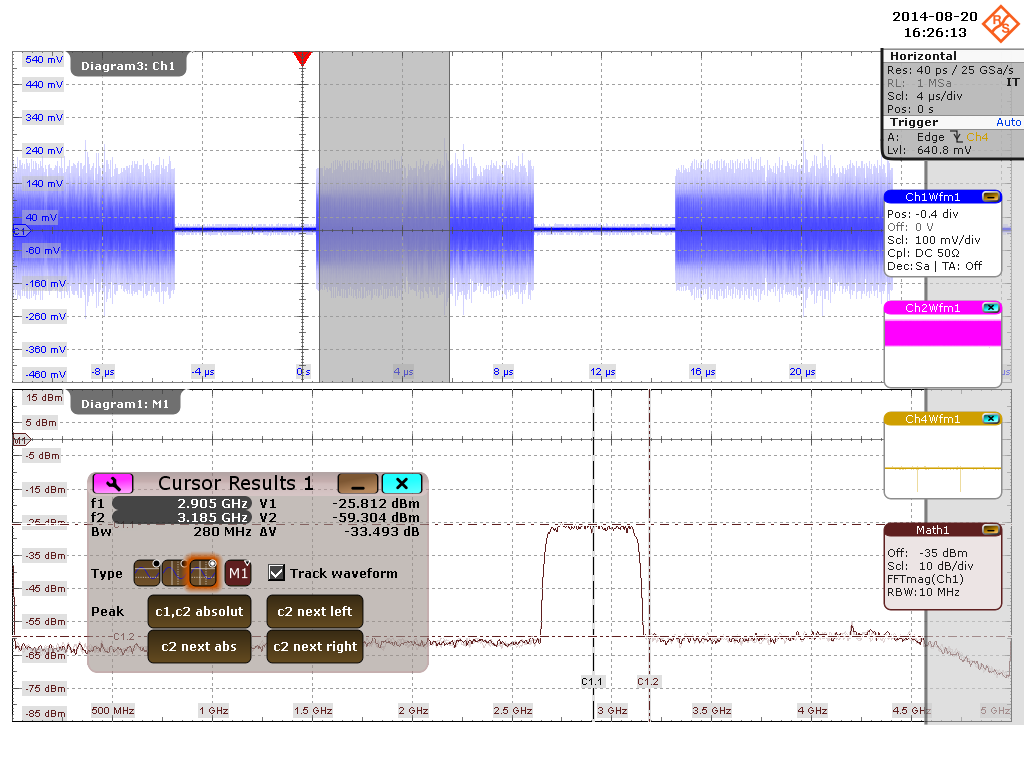
\includegraphics[width=\textwidth]{figures/osci/res_450_awg_analog}
  \caption{\gls{TX} \gls{IF} signal generated by the \gls{AWG}}
  \label{fig:res_450_awg_analog}
\end{figure}

\begin{figure}[p]
  \centering
  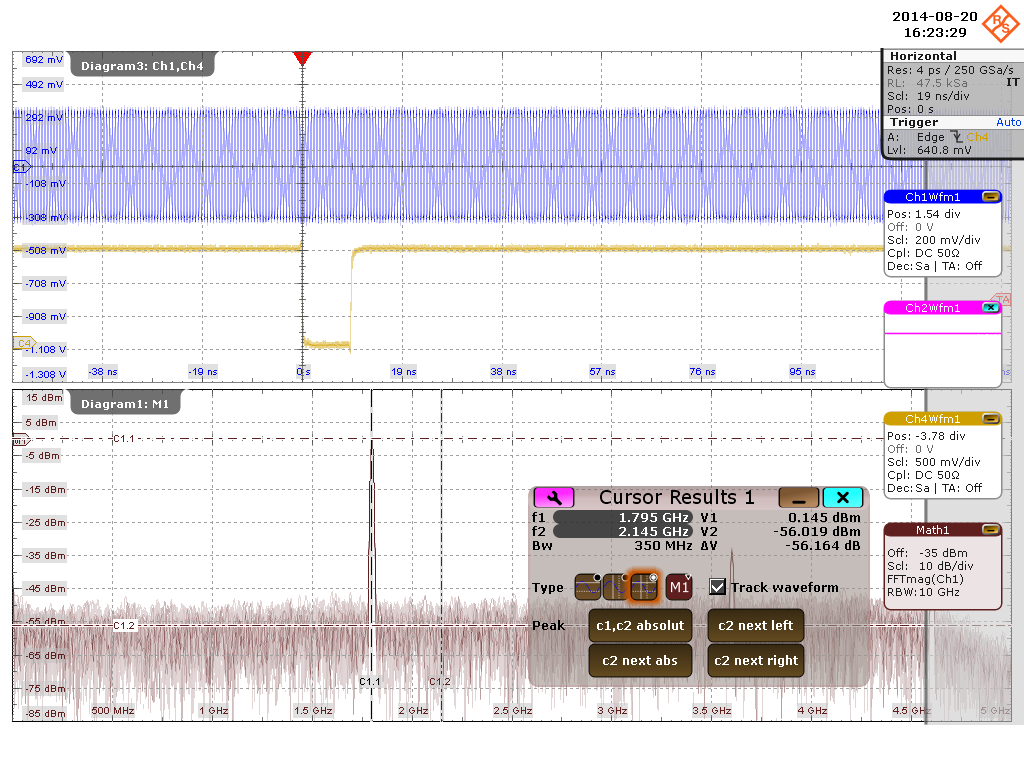
\includegraphics[width=\textwidth]{figures/osci/res_450_awg_digital}
  \caption{\gls{ADC} clock signal and sync pulse generated by the \gls{AWG}}
  \label{fig:res_450_awg_digital}
\end{figure}

\subsubsection{RF parts}
The two analog channels generated by the \gls{AWG} have a total signal
power of -9.28 dBm each \eqref{eq:res_450_awg_pwr}. These signals were
than attenuated by 20 dB to be below the 1-dB output compression point of 10 dBm
of the 60 GHz converters even at full gain of 40 dB. \\

\begin{align}
  10 \cdot \log_{10}\left(
  10^{-25.812 \;\text{dBm} / 10} \cdot
  \frac{450 \;\text{MHz}}{10 \;\text{MHz}}
  \right) \approx -9.28 \;\;\text{dBm}
  \label{eq:res_450_awg_pwr}
\end{align}

The same 60 GHz converter was used for transmission and reception and
configured as shown in \tblref{tab:res_450_sivers} (configuration script
see \appref{app:}).
A 10 MHz reference clock was fed from the \gls{AWG}.
An aluminium plate in a distance of about 15 cm was used as a reflector. \\

\begin{table}[h]
  \centering
  \begin{tabular}{|l|l|}
    \hline
    Reference Clock & external \\ \hline
    TX Oscillator Frequency & 57.5 GHz (0x038170) \\ \hline
    RX Oscillator Frequency & 58.2 GHz (0x038D60) \\ \hline
    TX Power & 0x80 \\ \hline
  \end{tabular}
  \caption{Configuration Parameters of 60 GHz Converter}
  \label{tab:res_450}
\end{table}

Both channels on the \gls{RX} side of the converer first connect to a
\gls{MC} BHP-1000+ high-pass filter. As we can see in \figref{fig:res_450_rx_if},
the \gls{TX} \gls{LO} leackage is attenuated by about 35 dB. Also the \gls{TX}
\gls{LSBand} signal (centered around 3.6 GHz) is about 17 dB weaker than
the desired \gls{TX} \gls{USBand} signal. This is due to the transmitter's
image rejection and the fact that the \gls{LSBand} signal is outside the
\gls{RF} specification of the converter. \\

\begin{figure}[p]
  \centering
  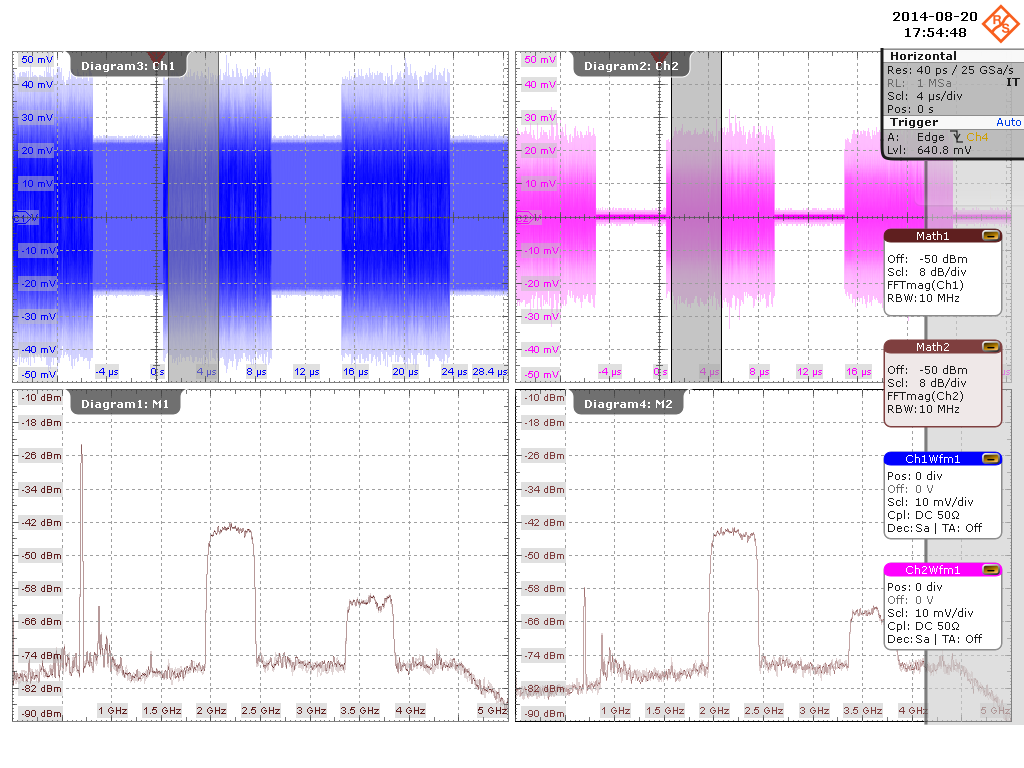
\includegraphics[width=\textwidth]{figures/osci/res_450_rx_if}
  \caption{Received \gls{IF} Signal before (left) and after (right) High-Pass Filter}
  \label{fig:res_450_rx_if}
\end{figure}p

Next the signal amplified by 12 dB to drive the \gls{ADC} input to about 70\%
as shown in \figref{fig:res_450_rx_amp}. \\

\begin{figure}[p]
  \centering
  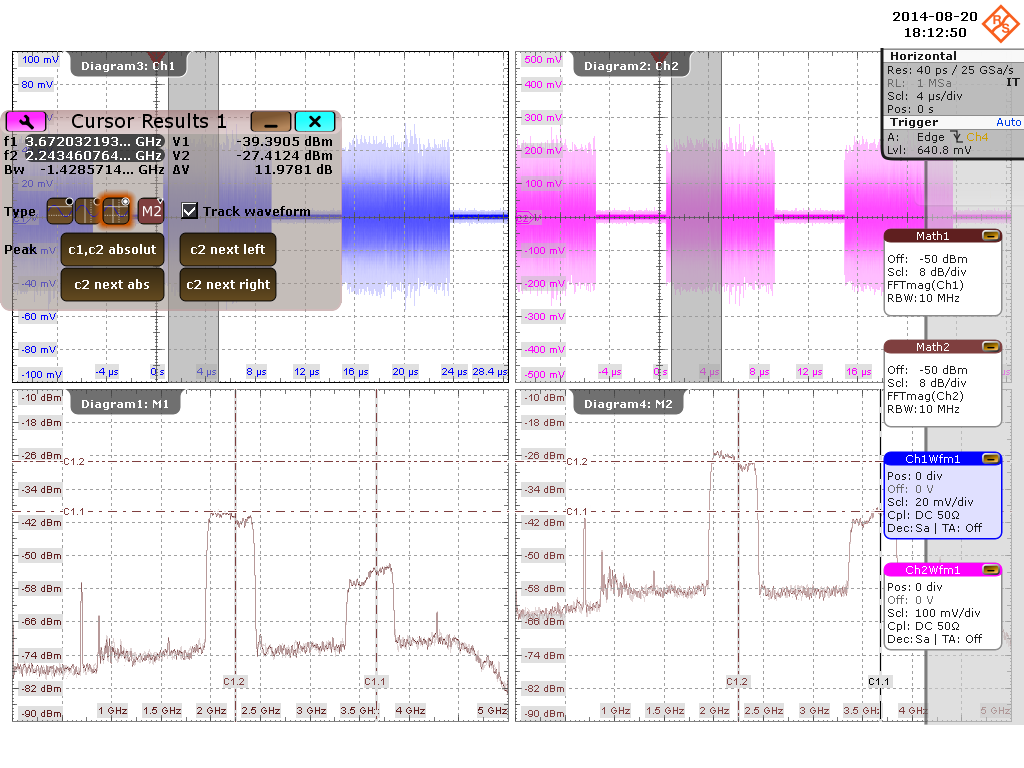
\includegraphics[width=\textwidth]{figures/osci/res_450_rx_amp}
  \caption{Received \gls{IF} Signal before (left) and after (right) the Amplifier}
  \label{fig:res_450_rx_amp}
\end{figure}

Finally the signal is converted to a differential signal using a ADC-WB-BB Balun
(\secref{sec:comp_balun}), passes a \gls{DC} block (\secref{sec:comp_dc_block})
and digitized by the \gls{ADC}. \\

The channel filter shown in \figref{fig:rx_2_bd} is therefor build using
the BHP-1000+ high-pass filter and the \gls{ADC} analog input bandwidth which
cuts of at about 2.8 GHz. \\

\section{Error Vector Magnitude Measurements}
Random Mean Error Vector Magnitude
Deteministic Mean Error Vector Magnitude

\subsection{Channel impulse response}
\begin{itemize}
\item Show typical channel impulse response of one reflector setup.
\item Show delay spread.
\end{itemize}

\subsection{Phase Noise measurements}
\begin{itemize}
\item Phase-Noise plot measured using many short frames, show that correction algorithm works
\end{itemize}

\subsection{High Modulation Rate}
\begin{itemize}
\item Show that high modulation rates and multi GB/s throughput is possible (\gls{QAM} 256?)
\end{itemize}

\section{Full Bandwidth Transmission}
\subsection{Transmitter Channel Imbalance}
\begin{itemize}
\item Show that transmitter channel imbalance is not an issue
\end{itemize}

\subsection{90deg Coupler Error Measurement and Correction}
\begin{itemize}
\item Show error introduced by non-perfect 90 deg coupler.
\item Show the best correction I will come up with
\item Compare to best result achieved by classical architecture (with additional mixer)
\end{itemize}

%%  LocalWords:  multi QAM Coupler coupler
